\newpage


\section[Grundlagen der Kryptografie - Kryptografische Verfahren und Algorithmen]{Grundlagen der \gls{kryptografie} - \glsdisp{kryptografie}{Kryptografische} Verfahren und \glspl{algorithmus}}\label{sec:grundlagen-der-kryptografie}


In der digitalen Welt spielt die \Gls{kryptografie} eine entscheidende Rolle. Sie sichert Informationen durch Ver- und Entschlüsselung, um Vertraulichkeit, Integrität und Authentizität zu gewährleisten.
\glsdisp{kryptografie}{kryptografische} \glspl{algorithmus} dienen als grundlegende Bausteine, um Daten in eine unlesbare Form zu bringen und nur autorisierten Empfängern zugänglich zu machen.
Dieser Abschnitt gibt einen Überblick über die Grundlagen der \Gls{kryptografie} und verschiedene Arten von \glspl{algorithmus}, die in Webanwendungen und in der Informationssicherheit verwendet werden.
Es vermittelt die Prinzipien und Konzepte, um das Verständnis für die Bedeutung und den Einsatz von \Gls{kryptografie} in der vernetzten Welt zu stärken.


\subsection[Symmetrische Verschlüsselungsalgorithmen]{Symmetrische \glsdisp{algorithmus}{Verschlüsselungsalgorithmen} - \acf{DES}}\label{subsec:symmetrsiche-algorithmen}
Bei symmetrischen Verschlüsselungsalgorithmen wird, wie in \autoref{fig:symmetricalEncoding}\autocite{Chapter211:online} dargestellt, derselbe Schlüssel zum Verschlüsseln und zum Entschlüsseln einer Nachricht verwendet.
Dies ermöglicht eine einfache und schnelle Kommunikation, führt jedoch dazu, dass die Geheimhaltung des Schlüssels schnell zu einer Sicherheitslücke führen kann.

\begin{figure}[htbp]
    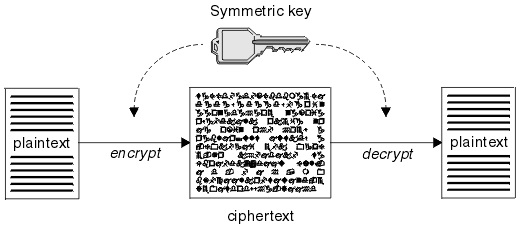
\includegraphics[width=1\linewidth]{abbildungen/symmetricEncoding}
    \centering
    \caption[
        Schaubild einer symmetrischen Verschlüsselung]{Schaubild einer symmetrischen Verschlüsselung\footnotemark}
    \label{fig:symmetricalEncoding}
\end{figure}
\footnotetext{\cite{Chapter211:online}}


Symmetrische Verschlüsselungsverfahren werden deshalb dann als sicher angesehen, wenn man ohne den Schlüssel den Klartext nicht aus dem verschlüsselten Text ermitteln kann.\autocite[\pagef~5]{kryptographische-algorithmen}

\ac{DES}, oft auch \ac{DEA}, wurde 1975 im \textit{Federal Register} der USA
veröffentlicht und als Kooperation zwischen dem \ac{NIST}, der \ac{NSA} und \ac{IBM} entwickelt.\autocite[\pagef~232]{nsa-meyer}

\ac{DES} ist ein Blockchiffre-Verfahren, was bedeutet, dass die Daten in immer gleich großen Blöcken, hier in Blöcken von 64 Zeichen, und mit einer immer gleichen Schlüssellänge, hier 56 Bit, verschlüsselt werden.\autocite[\pagef~6]{kryptographische-algorithmen}


\subsection[Asymmetrische Algorithmen]{Asymmetrische \glspl{algorithmus}}\label{subsec:asymmetrische-algorithmen}
Asymmetrische Verschlüsselungsverfahren verwenden, im Gegensatz zu den Symmetrischen (\solol), zwei Schlüssel.
Einen \gls{publicKey},zum Verschlüsseln der Daten und einen \gls{privateKey}, zum wieder Entschlüsseln.
Dabei muss ausschließlich der \gls{privateKey} geheim gehalten werden.


\subsubsection[RSA-Verfahren]{\acs{RSA}\nonbreakdash Verfahren}\label{subsubsec:rsa-verfahren}

\ac{RSA} ist das erste entwickelte \gls{publicKeyEncoding} und besitzt auch heute noch eine große Relevanz.\autocite[\pagef~168]{buchmann-einfuhrung-2016}

\paragraph[Schlüsselerzeugung]{Schlüsselerzeugung}\label{par:schluesselerzeugung}
Das generieren des \ac{RSA}-Schlüsselpaars benötigt einige verschiedene Zahlen.
Der Sicherheitsparameter $k \in \mathbb{N}$ gibt die Größe des Produkts der beiden gewählten Primzahlen für die Verschlüsselung an.
Zwei statistisch unabhängige, zufällige Primzahlen $p$ und $q$ werden ausgewählt, um den \ac{RSA}-Modul n zu bilden.
Dieser Wert wird später für Ver- und Entschlüsselung verwendet und berechnet sich als $n = p*q$.

Zusätzlich wird eine natürliche, ungerade Zahl $e$ gewählt, für die

\begin{equation}
    1 < e < \varphi(n) = (p - 1)(q - 1)\ \text{und}\ \gcd(e, (p-1)(q-1)) = 1\label{eq:equation2}
\end{equation}
gilt und daraus mit den folgenden Bedingungen
\begin{equation}
    1 < d < (p-1)(q-1)\ \text{und}\ d*e \equiv 1\mod(p-1)(q-1)\label{eq:equation3}
\end{equation}
eine weitere Zahl \(d \in \mathbb{N}\) gebildet.

Da $\gcd(e, (p-1)(q-1)) = 1$ gilt, existiert eine solche Zahl $d$ definitiv.
Berechnet werden kann sie mit dem \glspl{extendedEuklidAlgorithm}.
Der \gls{publicKey} bildet sich dabei aus dem Paar $(e, n)$, der \gls{privateKey} aus der Zahl $d$.\autocite[\pagef~169]{buchmann-einfuhrung-2016}

Damit \ac{RSA} eine sichere Verschlüsselung ermöglichen kann, müssen die beiden Primzahlen $p$ und $q$ passend gewählt werden.
Dafür ist es üblich, dass $k$ als eine gerade, mindestens $2^{10}$\nonbreakdash Bit lange Zahl gewählt wird.\autocite[\pagef~169]{buchmann-einfuhrung-2016}

\paragraph{Verschlüsselung}\label{par:verschluesselung}
Um mit dem \ac{RSA} \gls{algorithmus} eine Nachricht zu verschlüsseln, wird der \gls{publicKey} $(e, n)$ benötigt.
Aus einem \gls{klartext} \(m \in \mathbb{Z}_m\) mit \(\mathbb{Z}_m\) als \ac{RSA}\nonbreakdash\gls{klartextraum} erhält man den verschlüsselten Text $c$ mit
\begin{equation}
    c = m^e\mod n\label{eq:equation4}
\end{equation}
$m$ kann wieder rekonstruiert werden mit
\begin{equation}
    m = c^d \mod n\label{eq:equation5}
\end{equation}
wobei $c$ der zuvor erhaltene verschlüsselte Text, $d$ der \gls{privateKey} und $n$ ein Teil des \glsdisp{publicKey}{public Keys} ist.\autocite[\pagef~6]{rsa-encryption}

\subsubsection[Hashfunktionen]{Hashfunktionen — \acf{SHA}}\label{subsubsec:hash-funktion}
Im Grundlegenden sind Hashfunktionen \glspl{algorithmus}, die einen Text beliebiger Länge zu einem neuen Text mit vorgegebener Länge komprimieren\autocite[\pagef~15]{anal-des-hash-function-2003}.
Sie werden mithilfe von \sog \glspl{compressfunc} generiert.

Damit \glsdisp{hashfunc}{Hash}- und \glspl{compressfunc} in der \gls{kryptografie} zur Authentifizierung, wie \zb zur Speicherung von Passwörtern genutzt werden können, müssen sie noch verschiedene Kriterien erfüllen.
Diese werden folgend erklärt:

\begin{definition}[label=def:hashfunktion]
    Eine Einweghashfunktion ist eine Funktion $h$, die folgende Bedingungen erfüllt\autocite[\vglf][\pagef~17]{anal-des-hash-function-2003}:
    \begin{enumerate}
        \item Die Beschreibung von $h$ muss öffentlich bekannt sein und sollte keine geheimen Informationen erfordern (Erweiterung des Kerckhoff\textquotesingle schen Prinzips\autocite[]{petitcolas-information-nodate}).
        \item Das Argument $X$ kann von beliebiger Länge sein und das Ergebnis $h(X)$ hat eine feste Länge von $n$-Bits (mit $n \geq64$).
        \item Für gegebene $h$ und $X$, muss die Berechnung von $h(X)$ einfach\footnotemark sein.
        \item Die Hashfunktion muss in dem Sinne monodirektional sein, dass es bei einem $Y$ im Abbild von $h$ schwer\footnotemark[\value{footnote}] ist, aus einer Nachricht einen bestimmten \gls{hashwert} zu generieren, und dass es schwer\footnotemark[\value{footnote}] ist, zwei Nachrichten zu finden, die den gleichen \gls{hashwert} teilen.
    \end{enumerate}
    \footnotetext{\enquote{einfach} und \enquote{schwer} sind hier im kryptografischen Sinne zu verstehen und beziehen sich auf das Zusammenspiel von Laufzeit und Rechenaufwand eines \gls{algorithmus}\textquotesingle}
\end{definition}

\autoref{def:hashfunktion} verwendet die Begriffe \enquote{einfach} und \enquote{schwer}, da heutzutage noch keine \glspl{algorithmus} bekannt sind, die eine \glsdisp{hashfunc}{Einweghashfunktion} schnell genug umkehren können.\autocite[\pagef~234]{buchmann-einfuhrung-2016}

\acfp{SHA} sind verschiedene kryptologische Hashfunktionen und eine Modifikation des \gls{MD5}, welche zur Berechnung eines Prüfwertes für beliebige Nachrichten dienen und unter anderem die Grundlage zur Erstellung einer digitalen Signatur, genauer erläutert in \autoref{subsubsec:digitale-signaturen-und-zertifikate}, sind\autocite[]{WhatisSH81:online}.

2012 wurde \ac{SHA}-3\footnote{Auch als \textit{Keccak} bezeichnet}  von \ac{NIST} standardisiert und wird heute als sicher angesehen\autocite[\pagef~239]{buchmann-einfuhrung-2016}, aber auch die \glspl{algorithmus} unter \ac{SHA}-2 sind heute stark verbreitet.
\ac{SHA}-2 und \ac{SHA}-3 bezeichnen nicht einzelne \glspl{algorithmus} sondern \glsdisp{algorithmus}{Algorithmusgruppen}, deren zugrunde liegenden \glspl{algorithmus} sich primär in der Länge des ausgegebenen Prüfwertes unterscheiden.
Dabei werden die \glspl{algorithmus} \ac{SHA}-256 und \ac{SHA}-512 am häufigsten genutzt.